\chapter{高速Fourier変換(FFT)}
    \section{長さが2のべき乗でない信号のDFTを長さが2のべき乗の信号のFFTに帰着する方法}
        $N$を$2$のべき乗でない自然数とする。
        長さ$N$の信号$x$のDFT
        \[ X(k) = \frac{1}{\sqrt{N}} \sum_{n=0}^{N-1} x(n)\exp \left(2\pi i\frac{-kn}{N}\right) \quad k=1,2,\dots,N-1 \]
        を長さが$2$のべき乗である信号のFFTに帰着する方法を考える。
        $\forall a,b\in\mathbb{R},\;ab = \frac{a^2 + b^2 - (a-b)^2}{2}$を用いて上の式を次のように変形する。
        \begin{align*}
            \begin{aligned}
                X(k) &= \frac{1}{\sqrt{N}} \exp \left(\pi i\frac{-k^2}{N}\right) \sum_{n=0}^{N-1} x(n)\exp \left(\pi i\frac{-n^2}{N}\right) \exp \left(\pi i\frac{(k-n)^2}{N}\right) \\
                &= \frac{1}{\sqrt{N}} \exp \left(\pi i\frac{-k^2}{N}\right) \sum_{n=0}^{N-1} u(n)v(k-n) \\
                & \text{where} \quad u(n) \coloneq x(n)\exp \left(\pi i\frac{-n^2}{N}\right),\;v(n) \coloneq \exp \left(\pi i\frac{n^2}{N}\right)
            \end{aligned}
        \end{align*}
        \[ \therefore\; X(k)\sqrt{N} \exp \left(\pi i\frac{k^2}{N}\right) = (u*v)(k) \]
        $u*v$を,長さが$2$のべき乗の信号に対して使えるFFT, IFFTを用いて計算する。
        そのために長さが$2$のべき乗の信号同士の**巡回畳み込み**の中に$u*v$が部分的に現れるような状況を以下のようにして作り出す。
        \par
        $N_2 \coloneq \min\{a|\exists b\in \mathbb{N}, a = 2^b \geq 2N\}$ とする。
        長さ$N_2$の信号$u_2,v_2$を以下のように定義する。
        \[
            u_2(n) \coloneq \left\{
                \begin{aligned}
                    u(n) &\quad (n \in [0,N-1]) \\
                    0 &\quad (n \in [N,N_2-1])
                \end{aligned}
            \right.
        \]
        \[
            v_2(n) \coloneq \left\{
                \begin{aligned}
                    v(n) &\quad (n \in [0,N-1]) \\
                    0 &\quad (n\in [N,N_2-N]) \\
                    v(N_2-n) &\quad (n \in [N_2-N+1,N_2-1])
                \end{aligned}
            \right.
        \]
        $u_2$は$u$の後ろに$0$を並べて長さ$N_2$に拡張した信号である。
        $v_2$は長さ$N_2$の$0$が並んだ信号の前部を$v$で塗り替え,後部を$v$の第$1\sim N-1$要素をコピーして順番を逆にしたもので塗り替えた信号である。
        下の図は$u_2,v_2$を視覚的に表現したものである。
        \begin{figure}[H]
            \centering
            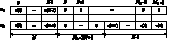
\includegraphics[keepaspectratio, scale=4]
            {parts/FourierSeries_and_FourierTransform/figs/FFT/arbitraryLengthFFT_to_powerOf2_FFT/u2,v2.pdf}
            \caption{$u_2,v_2$の構造}
        \end{figure}
        このようにすると$u_2*v_2$の先頭$N$要素が$u*v$と一致する。
        \[ \text{FFT}(u_2*v_2) = \sqrt{N_2}\text{ FFT}(u_2) \text{ FFT}(v_2) \]
        より
        \[ \text{IFFT}(\sqrt{N_2}\text{ FFT}(u_2) \text{ FFT}(v_2)) \]
        により$u_2*v_2$を高速に計算し,結果の先頭$N$要素を切り出せば$u*v$を得る。
        得られた$u*v$の第$k$要素に$\frac{1}{\sqrt{N}} \exp \left(\pi i\frac{-k^2}{N}\right)$を掛ければ$x$のDFTが得られる。
        $v_2$のFFTや$\frac{1}{\sqrt{N}} \exp \left(\pi i\frac{-k^2}{N}\right) \;(k=0,1,\dots,N-1)$は初回の計算結果を保存しておけば別の信号のDFTの計算で再利用できる。
